\chapter{Pengenalan Go}

\section{Apa itu Go?}

Go adalah nama bahasa pemrograman sekaligus nama implementasi dalam bentuk kompilator (\textit{compiler}). Untuk pembahasan berikutnya, istilah ``Go'' akan mengacu pada spesifikasi bahasa pemrograman serta peranti pengembangannya.

\section{Lisensi Go}

Go didistribusikan dengan menggunakan lisensi modifikasi dari BSD. Lisensi lengkap dari Go bisa diakses di \url{http://golang.org/LICENSE}. Secara umum, penggunaaan lisensi ini mempunyai implikasi sebagai berikut:
\begin{itemize}
\item boleh digunakan untuk keperluan komersial maupun non-komersial tanpa batasan
\item boleh memodifikasi sesuai keperluan
\item boleh mendistribusikan
\item boleh memberikan sublisensi ke pihak lain
\item boleh memberikan garansi
\item tidak boleh menggunakan merk dagang Go
\item tanpa jaminan dan jika terjadi kerusakan terkait penggunaan software ini maka pemberi lisensi tidak bisa dituntut
\item jika mendistribusikan harus mengikutsertakan pemberitahuan hak cipta.
\end{itemize}

\section{Instalasi Go}

Go tersedia pada berbagai platform. Proyek Go sendiri secara resmi mendukung platform Linux, FreeBSD, MacOSX, dan Windows. Dukungan tersebut merupakan dukungan resmi dan distribusi \textit{binary} dari berbagai platform tersebut tersedia di \url{https://code.google.com/p/go/downloads/list} seperti bisa dilihat di Gambar~\ref{fig:downloadGo}

  \begin{figure}
    \begin{center}
      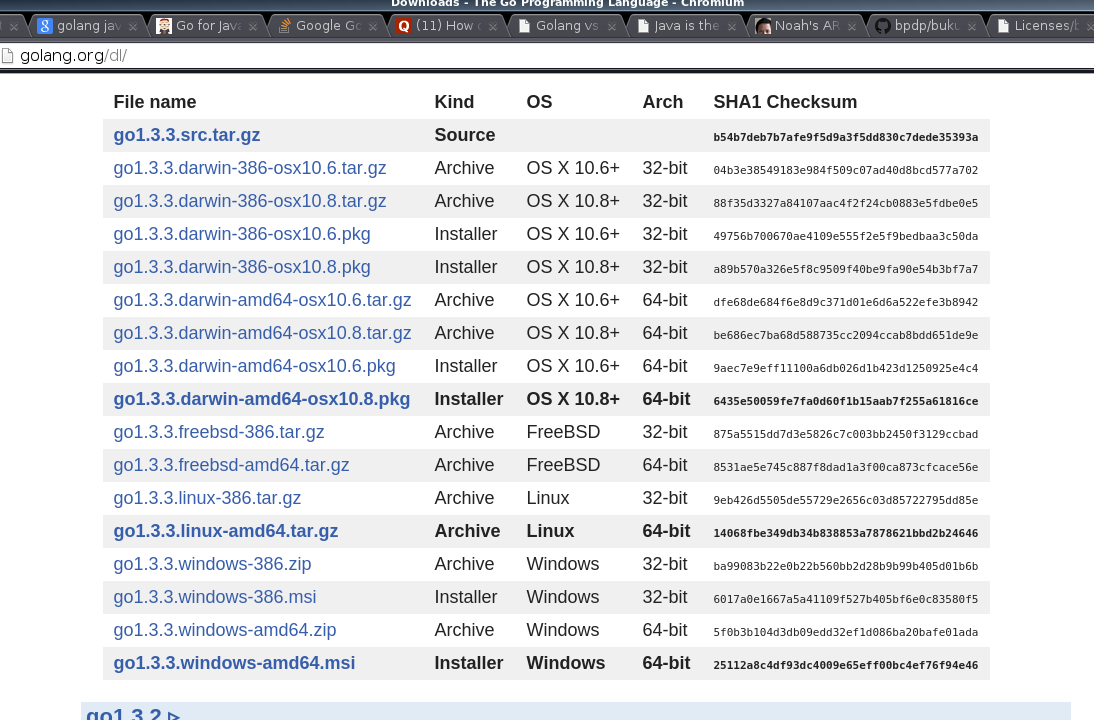
\includegraphics[scale=0.5]{images/download-go.png}
    \end{center}
		\caption{Distribusi \textit{binary} dari Go}
    \label{fig:downloadGo}
  \end{figure}

	Dengan dukungan tersebut, Proyek Go akan menerima laporan \textit{bugs} terkait dengan distribusi pada berbagai platform tersebut. Meski demikian, bukan berarti platform-platform lain tidak bisa menggunakan Go karena distribusi dalam bentuk kode sumber tersedia dan telah berhasil dikompilasi ke berbagai platform: NetBSD, OpenBSD, DragonFlyBSD, dan lain-lain\footnote{Lihat \url{http://go-lang.cat-v.org/os-ports}} untuk perkembangan dalam hal ini.


\subsection{Menguji Instalasi Go}

Kode sumber Go yang kita buat bisa dijalankan / dieksekusi tanpa harus dikompilasi (jadi seperti script Python atau Ruby) atau bisa juga dikompilasi lebih dulu untuk menghasilkan \textit{binary executable}\footnote{Catatan: selain ini sebenarnya ada paket pustaka yang dimaksudkan untuk digunakan dalam program, akan dibahas belakangan}. 

Untuk menguji, buat program sederhana seperti pada Listing~\ref{lst:helloGo}. Setelah itu, gunakan ``go run namafile.go'' untuk menjalankan secara langsung atau dikompilasi lebih dulu dengan ``go build namafile.go'' seperti pada Listing~\ref{lst:ujiGo}.
	
\lstset{language=Go, caption=hello.go, label={lst:helloGo}}
\lstinputlisting{src/go/bab-01/hello.go}

\lstset{language=bash, caption={Menguji instalasi Go di Linux}, label={lst:ujiGo}}
\lstinputlisting{src/non-go/bab-01/test-instalasi-go.txt}

\section{Memahami Lingkungan Peranti Pengembang Go}

Saat menginstall Go, kita akan memperoleh 3 buah file \textit{binary executable}:
\begin{itemize}
	\item \textbf{go}
	\item \textbf{godoc}
	\item \textbf{gofmt}
\end{itemize}

Penjelasan untuk masing-masing akan diuraikan di sub-sub bab berikut.

